% Author: Alfredo Sánchez Alberca (asalber@ceu.es)
\chapter{Introducction to Derive}

\section{Introduction}
In the last decades, the computational power of computers have converted them in powerful tools for disciplines that, as Mathematics, require a large amount of complex computations.

Derive$^{\textsf{\textregistered}}$
\renewcommand{\thefootnote}{\fnsymbol{footnote}}\footnote{These practices are based on version 6.1 of Derive$^{\textregistered}$ for Windows.} is one of the most used programs for doing numerical and symbolic computations.  

Beyond their capabilities for the numerical, vectorial and matrix calculus, it also makes graphical representations. 
This allows to solve a lot of problems of Algebra, Analysis, Calculus, Geometry and even Statistics. 
The advantage of Derive versus other software as Mathematica, Mapple or MATLAB, is its simplicity, what makes it suitable for teaching Maths. 

\begin{center}
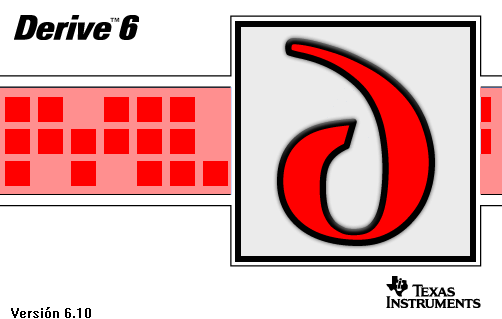
\includegraphics[scale=0.6]{img/introduction/introduction}
\end{center}


The goal of this practice is to introduce the basic usage of this program to the student. 


\section{Basic functionalities}
\subsection*{Starting the program}
As any other Windows applications, to start the program you have to click the \menu{Windows start} button and then select \menu{All the programs > Derive 6} or simply double click the desktop shortcut if there is one. 


\begin{center}
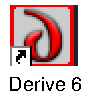
\includegraphics[scale=0.4]{img/introduction/derive_icon}
\end{center}

When the program starts, the main window, that is known as \emph{Algebra window} is shown (figure \ref{g:main}).

\begin{figure}[h!]
\begin{center}
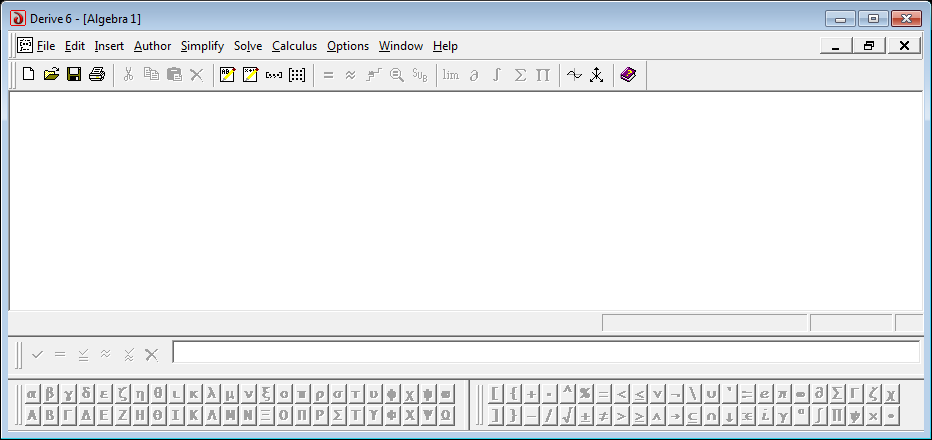
\includegraphics[width=\textwidth]{img/introduction/algebra_window}
\caption{Algebra window of Derive} \label{g:main} 
\end{center}
\end{figure}


The Algebra window has a title bar, a menu bar with menus for all the computations that Derive can performs (limits, derivatives, integrals, graphical representations, etc.), a tool bar with buttons for the main computations, the working area that contains the mathematical expressions that we are working with, the expression editor bar to enter mathematical expressions, the Greek letters and symbols button bar with Greek letters and symbols to enter in expressions and the status bar that shows what is the program doing at any moment. 

\subsection*{Expression edition}
Before doing any computation with a mathematical expression we have to enter it. 

\subsection*{Entering a mathematical expression}
To enter a mathematical expression we use the expression editor bar (figure~\ref{g:expression-editor}), that usually appears at the bottom of the Algebra widows, over the Greeks letters and symbols bar.

\begin{figure}[h!]
\begin{center}

\includegraphics[scale=0.6]{img/introduction/expression_editor}
\caption{Expression editor bar.} \label{g:expression-editor} 
\end{center} 
\end{figure}


In the expression editor bar we can write numbers, letters (that are variables) and symbols and arithmetic and logic operators. 
The most common operators are shown in the table below. 
You can also enter any Greek letter or symbol of the Greek letters and symbols button bar, just clicking on it.


\begin{center}
\begin{tabular}{cc}
\tcrule
\textbf{Symbol} & \textbf{Operator} \\
\texttt{+} & addition \\
\texttt{-} & subtraction \\
\texttt{*} & product \\
\texttt{/} & division \\
\texttt{\^{}} & power \\
\bcrule
\end{tabular}
\end{center}


Operators have different priorities when Derive evaluates a expression. 
First it evaluates functions and constants, second powers, third products and quotients (from left to right) and finally sums and subtractions (from left to right). 
You have to take into account this priority or use parenthesis to force a subexpression to be evaluated before the rest. 
In the following example you have different expressions and what Derive interprets for each of them

\begin{center}\renewcommand{\arraystretch}{2}
\begin{tabular}{cc}
\tcrule
\textbf{Entered expression} & \textbf{Evaluated expression} \\
\texttt{4x-1/x-5} & $4x-\dfrac{1}{x}-5$ \\
\texttt{(4x-1)/x-5} & $\dfrac{4x-1}{x}-5$ \\
\texttt{4x-1/(x-5)} & $4x-\dfrac{1}{x-5}$ \\
\texttt{(4x-1)/(x-5)} & $\dfrac{4x-1}{x-5}$ \\
\bcrule
\end{tabular}
\end{center}

After entering a expression and pressing \button{Enter}, the expression is shown in the working area of the Algebra window, labelled with a tag \verb"#" and a number, such as is shown in the figure~\ref{g:expressions}. 
After that we can reference that expression using its label instead of typing again the expression. 

We can select any expression of the Algebra window click on it. 
If you click several times on the same expression you can select different subexpressions. 
It is also possible to select several consecutive expressions in a block clicking on the first expression and dragging the cursor to the last. 

A useful key is \texttt{F3} that allow entering the selected expression or subexpression in the expression editor bar.

\subsubsection*{Modifying a expression}
Once a expression has been entered, we can modify it clicking on the expression and selecting the menu \menu{Edit > Expression}. 
The expression will be entered in the expression editor bar where you can change whatever you want. 
After making the changes, don't forget to press \button{Enter}. 

\subsubsection*{Removing expressions}
To remove a expression form the working area of the Algebra window, it is enough to select the expression and then press the \button{Supr} key or select the menu \menu{Edit > Delete}.
After removing a expression the labels of the other expressions are renumbered automatically. 
It is also possible to remove blocks of consecutive expressions. 

\textbf{Important!}: If we remove a expression by mistake, it is possible to recover it with the menu \menu{Edit > Undelete}.

\subsubsection*{Rearranging expressions}
It is possible to change the position of any expression in the working area of the Algebra window just clicking on it and, when the expression or block is selected, clicking again on it an dragging it to the new position.  
After arranging a expression the labels of the other expressions are renumbered automatically. 

\subsubsection*{Entering Comments}
The are two ways of entering comments in the working area of the Algebra window. 
The first one is in the expression editor bar, entering the text of the comment in double quotes.
If we proceed this way, the comment will be shown in the working area as any other expression, with its label. 
The second one is with the menu \menu{Insert > Text object}.
If we proceed this other way, the comment will be shown in the working area as an object without label. 

\subsubsection*{Naming variables}
By default Derive uses a single letter to represent variables. 
Thus, the expression \texttt{xy}, is not interpreted as a variable but as the product of variables $x$ and $y$.
Also by default, Derive does not distinguish between lowercase and uppercase letters.
For instance, Derive will interpret the same both if we write \command{cos(x)} or if we write \command{cos(X)}.
Nevertheless, it is possible to configure Derive to use more than one letter for variable names and to be case sensitive with the \menu{Options > Mode settings > Input}.

\subsubsection*{Defining constants and functions}
It is possible to define constants and functions with the operator \command{:=}.
To define a constant it is enough to type the name of the constant followed by \command{:=} and the value of the constant.
For example to define the gravitational constant we can write \command{g:=9.81}. 

To define a function, on the other hand, we have to type the name of the function followed by the list of variables separated by comma in brackets, then \command{:=} and the expression that defines the function. 
Thus, for instance, to define the function that measures the area of a triangle \command{a(b,h):=(b*h)/2} where \command{b} and \command{h} are the variables for the base and the height of the triangle respectively (see figure~\ref{g:expressions}).

With respect to the definition of constants and functions we must be aware of two important facts: 

\begin{itemize}
\item Any time we define a constant or function, the definition is active during all the working session, even if we remove the definition expression.
To remove a definition we have to redefine the constant or function but letting blank the expression after \command{:=}.
For example, to remove the definition of the gravitational constant we have to write \command{g:=}.

\item Derive is case sensitive to function names, so that \command{a(b,h)} and \command{A(b,h)} will be different functions.
\end{itemize}

\subsubsection*{Built-in constants and functions}
Derive has most of the constants and elementary functions used in Mathematics built-in. The syntax of some of them is shown in table ~\ref{t:elementary-functions}.

\begin{table}[h!]
\centering
\begin{tabular}{cl}
\tcrule
\textbf{Syntax} & \textbf{Constant or function} \\
\verb"#"\command{e} & Euler's number $e=2.71828\ldots$ \\
\command{pi} & The number $\pi=3.14159\ldots$ \\
\verb"#"\command{i} & The imaginary number $i=\sqrt{-1}$ \\
\command{inf} & Infinite $\infty$ \\
\command{exp(x)}  & Exponential function $e^x$ \\
\command{log(x,a)} & Logarithmic function with base $a$, $\log_a x$ \\
\command{ln(x)} & Natural logarithmic function $\ln x$ \\
\command{sqrt(x)} & Square root function $\sqrt{x}$ \\
\command{sin(x)} & Sine function $\sin x$ \\
\command{cos(x)} & Cosine function $\cos x$ \\
\command{tan(x)} & Tangent function $\tan x$ \\
\command{asin(x)} & Arcsine function $\arcsin x$ \\
\command{acos(x)} & Arccosine function $\arccos x$ \\
\command{atan(x)} & Arctangent function $\arctan x$ \\
\bcrule
\end{tabular}
\caption{Syntax of some predefined constants and functions.} \label{t:elementary-functions}
\end{table}

In some cases we can also use the symbols of the symbols button bar to refer to these constants.

To know all the built-in constants and functions of Derive we can use the menu \menu{Help > Online} and visit the section \textsf{Built-in Functions and Constants}.

\textbf{Important!}: In built-in functions Derive is not case sensitive.
For instance, the cosine function can be written \command{cos(x)}, \command{Cos(x)} or \command{COS(x)}.

\subsubsection*{Vectors and matrices}
Derive can also deal with vectors and matrices.
To enter a vector you can use the menu \menu{Author > Vector}.
Then enter the number of elements of the vector in the dialog shown and click the \button{OK} button. 
Finally enter the elements of the vector in the dialog shown and click again the \button{OK} button. 
Another way to enter vectors in the expression editor bar is to type their components separated by commas in square brackets. 
For instance, to enter the vector $(x,y,z)$ we write \command{[x,y,z]} (see the figure~\ref{g:expressions}).

To enter matrices we can use the menu \menu{Author > Matrix}.
Then enter the number of rows and columns of the matrix in the dialog shown and click the \button{OK} button. 
Finally enter the elements of the matrix in the dialog shown and click again the \button{OK} button. 

Another way to enter matrices in the expression editor bar is to type their row vectors separated by commas in square brackets. 
For instance, to enter the matrix
\[
\left(
\begin{array}{ccc}
 1 & 2 & 3 \\
 a & b & c \\
\end{array}
\right)
\]
we write \command{[[1,2,3],[a,b,c]]} (see the figure~\ref{g:expressions}).

\begin{figure}[h!]
\begin{center}
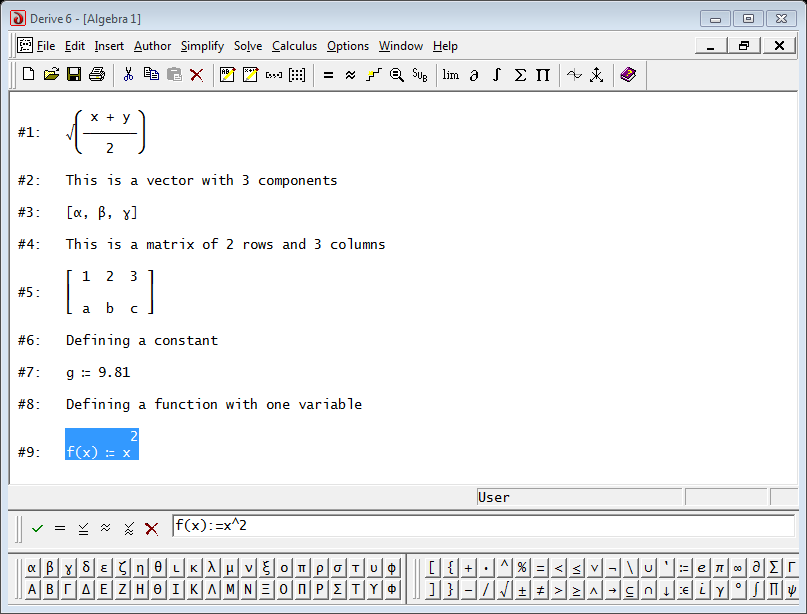
\includegraphics[width=0.8\textwidth]{img/introduction/expressions}
\caption{Different types of expressions in the Algebra window.}
\label{g:expressions}
\end{center}
\end{figure}


\subsection*{Simplifying expressions}
Derive has several ways to simplify expressions.
The simplest one is the basic simplification, that can be done with the menu \menu{Simplify > Basic}. 
This menu performs basic simplifications as, for instance, convert the expression $x+x$ in the expression $2x$. 
However, it doesn't allow to convert the binomial $(x+1)^2$ in $x^2+2x+1$, as it is not clear what of these expressions is simpler. 

To get the expansion of this binomial we can use the menu \menu{Simplify > Expand} that allow to expand a expression with respect to its variables.

On the contrary, if we want to get the binomial from the expanded form, we can use the menu \menu{Simplify > Factor} that allows to factor a expression with respect to its variables.

In any of these simplification types Derive woks in exact mode, what means that decimal numbers are expressed as fractions. 
To get the approximate value of an expression in a decimal form you can use the menu \menu{Simplify > Approximate}. 
This menu shows a dialog where we have to enter the number of decimal places that we want.

Finally, in any expression it is possible to substitute any variable by a value with the menu \menu{Simplify > Variable substitution}.
In the dialog shown you have to select the variable to substitute, enter the value for that variable in the field \field{New value} and click the button \button{OK}.


\subsection*{Graphical representations}
Derive can plot graphical representations in 2 and 3 dimensions.

\subsubsection*{2-dimensional graphical representations}
To represent a function or expression with one variable, we have to select the expression and then the menu \menu{Window > New 2D-plot window}.
This will open a new graphic window with two Cartesian axes ($x$ and $y$).
Finally, to show the graph of the expression in the Cartesian plane you have to select the menu \menu{Insert > Plot} or just click the corresponding button in the toolbar. 
Figure~\ref{g:2d-plot} shows an example of a 2-dimensional plot.

\begin{figure}[h!]
\begin{center}
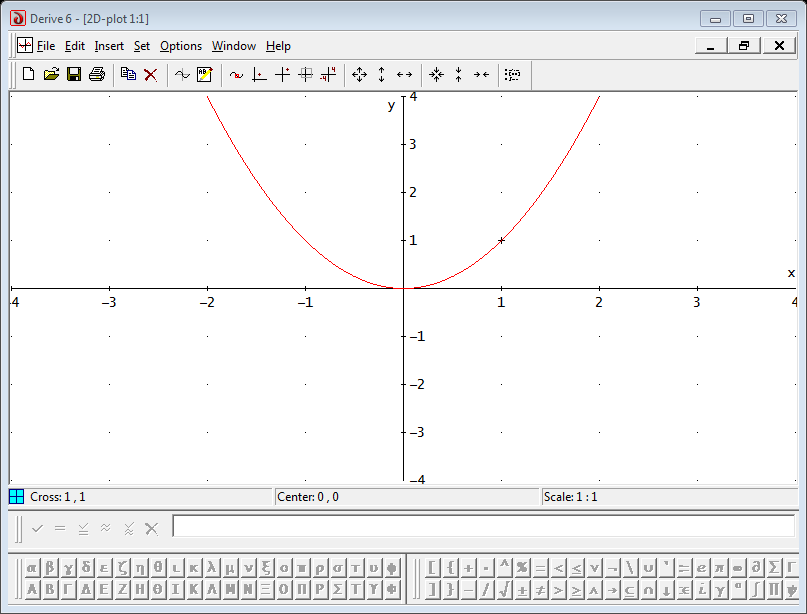
\includegraphics[width=0.8\textwidth]{img/introduction/2d-plot}
\caption{2-dimensional graphic window with the graph of a function.}
\label{g:2d-plot}
\end{center}
\end{figure}

If we want to show the plot in the Algebra window we can use the menu \menu{File > Embed}.

It is possible to represent more than one function in the same 2-dimensional graphic window. 

You can change from the Algebra window to the graphic window and vice versa selecting the corresponding window in the menu \menu{Window}.
However, when you are plotting several expressions is better to see the Algebra and graphic windows at the same time using the \menu{Window > Tile Vertically} (see figure~\ref{g:algebra-2d-plot}.

\begin{figure}[h!]
\begin{center}
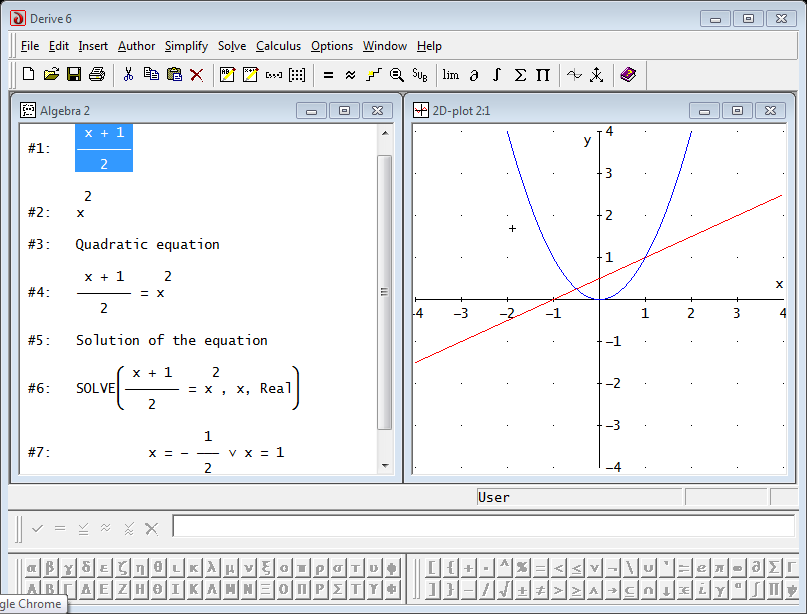
\includegraphics[width=0.8\textwidth]{img/introduction/algebra_2d-plot}
\caption{An Algebra and a 2-dimensional graphic window showed at the same time.} 
\label{g:algebra-2d-plot}
\end{center}
\end{figure}

\subsubsection*{Removing a plot}
To remove the last plot from a graphic window you can use the menu \menu{Edit > Delete plot > Last}. 
It is also possible to remove the first and all the plots but the last with the corresponding menus. 

\subsubsection*{Scaling a plot}
In the graphic window there are several menus and buttons to change the aspect of the plots. 

One of the most interesting actions is changing the scale of axes with the menu \menu{Set > Aspect Ratio}.
It is also possible to change the visible area of the plot with the menu \menu{Set > Plot Range > Minimum/Maximum}. 
In the dialog shown you have to enter the minimum and maximum values for every axis and click the button \button{OK}.


\subsubsection*{Tracing a plot}

In the 2-dimensional graphic windows there is a small cross that we change of position just clicking on a new position of the graphic window.
The coordinates of the cross are always shown in the bottom-left corner of the status bar.
If you press the \command{F3} key, the cross changes to a small square and passes to the \emph{trace mode}.
In this mode the square follows the trajectory of a graph using the arrow keys of the keyboard.
Use the left/right arrows to move the square to the left/right respectively and the up/down arrow to change the graph to follow when there are more than one plot. 
This can be helpful to see the value that takes a function in the graphic window or the points where two graphs intersect (see figure~\ref{g:trace-mode}.

\begin{figure}[h!]
\begin{center}
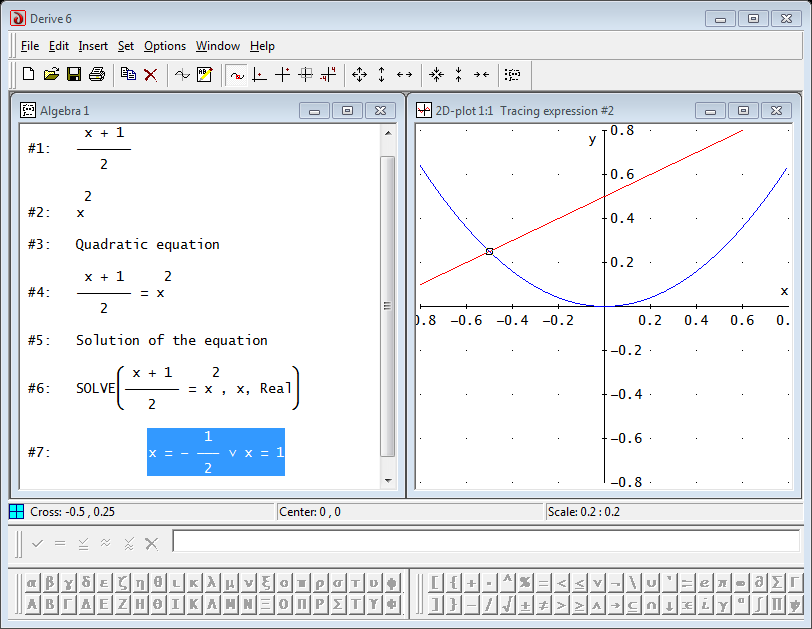
\includegraphics[width=0.8\textwidth]{img/introduction/trace_mode}
\caption{Graphic window in trace mode showing the point where two graphs intersect (that is one solution of the equation).}
\label{g:trace-mode}
\end{center}
\end{figure}


\subsubsection*{Centering the plot}
It is also possible to center the plot at the position of the cross with the button \button{Center on Cross} or at the origin of coordinates with the button \button{Center on Origin}.


\subsubsection*{2-dimensional graphical representations}
To represent a function or expression with 2 variables we have to select the expression and then the menu \menu{Window > New 3D-plot window}.
This will open a new graphic window with three Cartesian axes ($x$, $y$ and $z$).
Finally, to show the graph of the expression in the Cartesian space you have to select the menu \menu{Insert > Plot} or just click the corresponding button in the toolbar. 
Figure~\ref{g:3d-plot} shows an example of a 3-dimensional plot.

\begin{figure}[h!]
\begin{center}
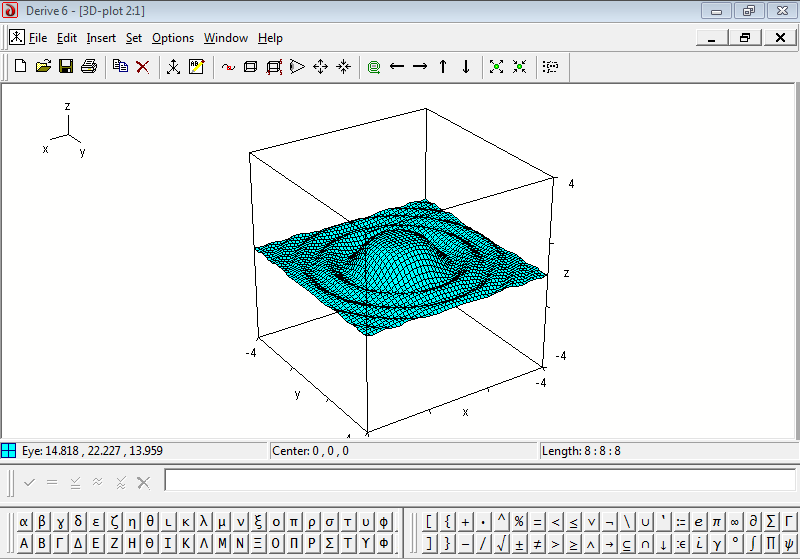
\includegraphics[scale=0.6]{img/introduction/3d-plot}
\caption{3-dimensional graphic window with the graph of a function.}
\label{g:3d-plot}
\end{center}
\end{figure}

Again it is possible to represent more than one function in the same 3-dimensional graphic window. 

Like for 2-dimensional graphic windows, there are several menus an buttons to change the aspect of the plot.

\subsubsection*{Changing the perspective of the plot}
One of the most interesting actions is changing the perspective of the plot with the menu \menu{Set > Eye Position}.
In the dialog shown you have to enter the coordinates of the observer eye and click the button \button{OK}.
It is also possible to change the perspective of the plot rotating the plot horizontally with the left/right arrow keys or vertically with the up/down arrow keys. 

\subsubsection*{Changing the resolution of the grid}
Derive plots the surfaces with a grid of small tiles. 
To change the resolution of the grid you can use the menu \menu{Edit > Plot}. 
In the dialog shown you can enter the number of vertical and horizontal panels.
The higher the number of panels the smoother the surface. 


\subsection*{File management}
The expressions and computations of an Algebra windows can be saved in a file.

\subsubsection*{Saving a file}
To save the content of an Algebra window in a file you can use the menu \menu{File > Save}.
In the dialog shown give a name to the file, select the folder where to save it and click the button \button{Save}.
Derive will put automatically extension \texttt{*.dfw} to the saved file. 
Once the file has been saved, its name will be shown in the title bar of the window. 


\subsubsection*{Opening a file}
To open a Derive file in an Algebra windows you can use the menu \menu{File > Open}.
In the dialog shown you only have to select the file that you want to open an click the button \button{Open}.
The selected file will be opened in a new Algebra window.


\subsubsection*{Opening and closing new Algebra windows}
Derive can manage more than one Algebra windows simultaneously. 
To open a new Algebra window you can use the menu \menu{File > New}. 
Derive works with each Algebra window independently.
That means that we can use the same names to refer to different constants or functions in different Algebra windows without interference. 

On the other side, to close an Algebra window you only have to use the menu 
\menu{File > Close}.


\subsubsection*{Printing}
To print the content of an Algebra window you can use the menu \menu{File > Print}.
However, before printing it is a good idea to preview the document with the menu 
\menu{File > Print Preview}. 
If everything is OK it is enough to click on the button \button{Print} to send the document to the printer. 
To change the margins and the orientation of the page you can use the menu \menu{File > Page Setup}.

Other options like the font, the header or the footer of the page can be set with the menu \menu{Options > Printing > Header and Footer}.


\subsubsection*{Getting help}
Like most Windows applications you can get help about the use of the program with the menu \menu{Help}.
